\documentclass[usletter]{article}
\usepackage{graphicx}
\usepackage{amsfonts}
\usepackage{amsthm}
\usepackage{amsmath}
\usepackage{amssymb}
\usepackage{scribe}
\usepackage[margin=1.5in]{geometry}

\begin{document}


\makeheader{Siddharth Joshi}      % your name
           {April 15, 2019}                   % lecture date
           {5}                                       % lecture number
           {Rank Bound v/s Fooling Set and the Log-Rank Conjecture}  % lecture title

\noindent
In the previous lecture we were introduced to the \emph{Rank-Bound Technique} which was shown to be more powerful than the earlier \emph {Fooling Set Technique} due to its ability to prove a tight lower bound for the \emph{Inner Product} function as well as for the ease with which it allowed for bounds on the deterministic communication complexity of the \emph{Greater-Than} and \emph {Set Disjointness} functions. It was presented as effectively a characterization of deterministic communication. \newline

This lecture begins with a solution to Challenge Problem 4 which dealt with the relation of the Rank over Arbitrary Fields v/s the Reals, and this result helps us move towards a better understanding of how rank varies across fields (which will prove to be useful in our usage of the Rank-Bound Technique to prove various bounds). This is followed by a discussion of Challenge Problem 5 that necessitates the proving of an interesting theorem that shows that the largest fooling set in a matrix is at most the rank of the matrix in any field (thus it is at most the minimum rank of the matrix in any field). The theorem intends to formalize the notion of the \emph {Rank-Bound Technique} being relative more powerful by providing tighter lower bounds than the \emph {Fooling-Set Technique}, and thus convinces us of the utility of the \emph {Rank-Bound Technique}. The result of this theorem in conjunction with the result from the previous lecture regarding the rank of \emph {Inner Product} function in $F_2$, finally enable to prove the statement of Challenge Problem 5 that shows us that the inability to find a large fooling set for the \emph {Inner Product} function was in the nature of things 9there is no such large fooling set). The discussion then moves to one of the most famous open problems in Communication Complexity: the \emph {Log Rank Conjecture} and then introduces an important fact about the communication complexity of the \emph {Unique Set Disjointness} predicate in order to demonstrate the limitations of the \emph {Rank-Bound Technique}. The lecture then concludes with Challenge Problem 6 (a solution for it has also been included). 

\section{Rank over Arbitrary Fields v/s Reals (Solution to Challenge Problem 4)}
\begin{lemma}
Let F and K be two fields such that F is a subfield of K (i.e. set theoretically F is a subset of K that satisfies the property of closure) then for all matrices $M \in F ^ {n \times m}$
$$ rk_{F} M = rk_{K} M $$

\end{lemma}

\noindent This lemma is particularly interesting as the truth of the statement may not be immediately obvious. In particular the rank of a matrix is simply the number of linearly independent columns or rows in it and enlarging the field significantly increases the number of linear combinations thus it is potentially possible to construct a set of vectors that are independent over F but dependent over K.
\begin{proof}
The proof is not too challenging, it relies simply on the understanding that elementary row operations that help get a matrix's reduced row echelon form do not alter rank. \newline
Let $r = rk_F M $ and $I_r = $ the identity matrix of size r $\times$ r. 
Then the reduced row-echelon form of M (represented in block matrix form below) using elementary row operations must be: \footnote {* - used to represent any arbitrary values for that block}
\[
\left(\begin{array}{@{}c|c@{}}
I_r & * \\
\hline
  0 & 0
\end{array}\right)
\]

And this concludes the proof as this new matrix is a matrix over K as well and the rank is by definition r. The original matrix can be recovered simply by using elementary row operations and it is possible to do so as F is a subfield not merely a subset and maintains closure over the operations used in elementary row operations, thus as such these elementary row operations are in some sense the  \lq inverse\rq of the ones we applied to obtain the row reduced echelon form. QED
\end{proof}

\begin{theorem}
For all fields F and M $\in \{ 0, 1\} ^ {n \times m}$
$$rk_F M \leq rk_{\mathbb{R}} M = rk_Q M $$
\end{theorem}

\begin{proof}
The trick to the proof lies in understanding the lemma and utilizing this to show that since Q is a subfield of $\mathbb{R}$ and hence $rk_{\mathbb{R}} M = rk_Q M $, it is equally valid to prove the theorem by working over the rational numbers. This is helpful as there doesn't seem to be any intuitive way to relate arbitrary fields to $\mathbb{R}$ (a field with characteristic zero), but working with the rational numbers allows us to come up with a very natural homomorphism that takes an arbitrary integer and relates it to an element in the field F (the homomorphism is simply adding 1 n times to obtain the integer n in question, this is always true as every field must have a multiplicative identity thus will contain 1). The main idea of the proof now is to use this understanding to show that if a set of boolean vectors are linearly dependent over Q, they are linearly dependent over F as well. \newline

\noindent Let $v_1, v_2$, ... ,$v_r$ be rows of M (therefore some arbitrary boolean vectors) \newline

\noindent If $v_1, v_2$, ... ,$v_r$ are linearly dependent over Q $\implies$ \newline

\noindent $\exists \; \lambda_1$, ... ,$\lambda_r$ such that $\lambda_1 v_1$ +  ... + $\lambda_rv_r$ = 0 such that $\lambda_1$, ... ,$\lambda_r$ are not all equal to 0\newline

\noindent From this we must now deduce that these vectors are also linearly dependent over the field F \newline

\noindent Without loss of generality, it can be assumed that $\lambda_1$, ... ,$\lambda_r$ are relatively prime integers as if not they can be trivially converted into relatively prime integers in the following manner: if the numbers are not already integers multiply through by the denominator and if they aren't relatively prime i.e. gcd $(\lambda_1$, ... ,$\lambda_r) \neq 1$ divide throughout by the common factor. (This doesn't in any way alter the vectors hence doesn't affect their linear dependence).\newline

\noindent The fact that $\lambda_1$, ... ,$\lambda_r$ are relatively prime $\implies$ that they are not all equal to $0_F$ as there exist $\alpha_1$, ... ,$\alpha_r \in \mathbb{Z}$ such that $\alpha_1 \lambda_{1_F}$ + ... + $\alpha_r \lambda{r_F} = 1_F$. Thus if $\lambda_1$, ... ,$\lambda_r$ were all to be $0_F$ it would lead to a contradiction. But if $\lambda_{1_F}$, ... ,$\lambda_{r_F}$ are not all equal to 0 then $v_1, v_2$, ... ,$v_r$ are linearly dependent in F as well.\newline

\noindent To conclude, we proved that any set of vectors $v_1, v_2$, ... ,$v_r$ that are linearly dependent in Q must be linearly dependent in an arbitrary field F as well thus, $rk_F M \leq rk_Q M$ but $rk_Q M =  rk_{\mathbb{R}} M$ by lemma 5.1, therefore $rk_F M \leq rk_{\mathbb{R}} M$. QED
\end{proof}

\section{Rank-Bound v/s Fooling Sets (Solution to Challenge Problem 5)}
This challenge problem asked to prove that the largest fooling set for the inner product function: $IP_n: \{0, 1\}^n \times \{0, 1\}^n \rightarrow \{0, 1\}$ is polynomial in n (the size of the input) and thus can't be used to obtain a tight bound for the communication complexity of the inner product function and hence dealt with the task of showing the relative strength of the \emph{Rank-Bound Technique} over the \emph {Fooling-Set Technique}. To achieve this however we must first prove an upper bound on the size of the largest fooling set and in some sense show the exponential gap that exists between this method and the \emph{Rank-Bound Technique}. The key idea here was to tackle the problem was to prove a general upper bound that must be true for any field F and exploit this to use the low rank of the characteristic matrix of the \emph{Inner Product} function in $F_2$ (as seen in the previous lecture) to bound the largest fooling set that can exist for it. The theorem thus presented introduces a general bound for the size of the largest fooling set of a matrix in terms of its rank in an arbitrary field. 

\begin {theorem}
For all fields F and all communication problems f 
$$f_s(f) \leq {(1 + rk_F M_f )}^2$$
\end{theorem}

\begin{proof}
The idea of the proof is to show that having a large fooling set i.e. exponential in n indicates a lot of structure (that functions like inner product do not have). In particular, the proof attempts to demonstrate that the bound given by the fooling set technique is only as good as the worst possible choice of field i.e the size of the largest fooling set is at most the minimum rank of the $M_f$ in any field F. This is done by using the notions of entry-wise product and tensor product discussed in earlier lectures to bound the size of the fooling set. \newline

\noindent Let S be a fooling set of $M_{IP_n}$ = $\{(x_1, y_1), ... , (x_s, y_s)\} \subset X \times Y $ \newline

\noindent Let s = $\lvert S \rvert$ \newline

\noindent \emph{Case 1: f(S) = 1} \newline

\noindent Let M = ${[ f(x_i, y_j) ]}_{\substack {i = 1 ... s \\ j = 1 ... s}}$ a submatrix of the characteristic matrix $M_{f}$ \newline

\noindent But since M is a fooling set the diagonal contains all 1s and the cross pairs of two entries on the diagonal cannot both be 1. Interpreting this mathematically $\implies M \odot M^T = I_s$ \newline

\noindent But $M \odot M^T$  is a sub-matrix of $M \otimes M^T$, thus for any field F $rk_F (M \odot M^T) = s \leq rk_F (M \otimes M^T)$ \newline

\noindent $\because  rk_F (M \otimes M^T) =  rk_F M  \dot rk_F M^T = {(rk_F M)}^2 \leq {(rk_F M_f)}^2 $ as M is a submatrix of $M_f$ \newline

\noindent $\therefore s \leq {(rk_F M_f)}^2 $ \newline

\noindent \emph{Case 1: f(S) = 0} \newline

\noindent This case can be resolved by using the result from Case 1. We must simply try and transform $M_f$ such that its rank does not change significantly but the 0-fooling set becomes a 1-fooling set for the new matrix. This can be done by taking the \lq complement \rq \footnote {the complement of the matrix M has been denoted by ${M_f}^c$} of the matrix in some sense. \newline

\noindent Let $J_s$ be the matrix of size s $\times$ s that has all entries = 1 \newline

\noindent $\therefore s \leq {(rk_F {M_f}^c)}^2 = {(rk_F (J_s - M_f))}^2 = {(1 + rk_F M_f)}^2$. QED

\end{proof}

\begin {problem}
Prove that for the inner product function: $IP_n: \{0, 1\}^n \times \{0, 1\}^n \rightarrow \{0, 1\}$
$$f_s(IP_n) \leq poly(n)$$
\end{problem}

\begin{proof}
\noindent The solution to the challenge problem is fairly easy after using the result proved in theorem 5.3. Using the fooling set of size n constructed in the previous lecture in the field $F_2$ it is easy to show an even stronger statement. \newline

\noindent By Theorem 5.3, $f_s(IP_n) \leq  {(1 + rk_F M_f)}^2$ for any field F. \newline

\noindent Thus setting F = $F_2$, $rk_{F_2} M_f \leq n$ as shown in the previous lecture. \newline

\noindent $\therefore f_s(IP_n) \leq {(1 +n)}^2 \implies f_s(IP_n) \leq poly(n)$. QED

\end{proof}

\noindent From theorem 5.3 and its application in problem 5.4 (Challenge Problem 5) it is evident that the \emph{Rank-Bound Technique} is significantly more powerful than the \emph {Fooling Set Technique}. Moreover coupled with the theorem presented in the previous lecture indicating its effectiveness for lower bounds on random communication problems, it can be considered to be in some sense a near-characterization of deterministic communication complexity (the next section on the log rank conjecture illustrates why the bound obtained may not always be tight and hence the technique may not actually be a complete characterization). The fooling set method then while effective for relatively simple functions like \emph{Equality} and \emph {Greater-than} immediately, and after some effort successful for the \emph {Set Disjointness} function as well, is shown to be far more limited in its application due to the amount of structure it requires in a problem. For a large fooling set for a function f to exist the rank of the characteristic matrix must be large in every field as the fooling set method is only as large as the rank of the characteristic matrix in the worst possible choice of field (as shown by theorem 5.3). On the other hand, the \emph {Rank-Bound Technique} is analogously as good as the best choice of field and the exponential gap between rank across fields shown as in the case of the \emph {Inner Product} function shows us how much the difference in choice of field can affect the bounds obtained. 

\section{Log Rank Conjecture}
This section introduces the log rank conjecture and illustrates the limitations of the \emph {Rank-Bound Technique} using a related result. 

\begin {conjecture}
For some constant c and all communication problems f 
$$ log (rk M_f) \leq D(f) \leq {(log (rk M_f))}^c + k $$
\end {conjecture}

\begin{remark}
This conjecture is perhaps the most important unsolved problem in the field of Communication Complexity and while there is overwhelming evidence supporting the upper bound conjectured, there is still no proof for it. It has been shown (as we will see in theorem 5.9) that c $\geq log(3)$, but nothing stronger has been proven. 
\end{remark}

\begin{fact}
Unique Set Disjointness Problem \newline
On input S, T $\subset \{1, ... ,n\}$ with $\lvert S \cap T \rvert \leq 1$ it takes $\Omega(n)$ bits of communication to computer DISJ(S, T). 
\end{fact}

\begin{remark}
The fact above refers not simply to a singular function but a family of functions that correctly compute the \emph{Unique Set Disjointness} predicate on inputs with at most 1 element in their intersection and are allowed to output anything when this condition is not met. \newline
The result is particularly interesting as despite the weakening by allowing the function to arbitrarily output any bit when $\lvert S \cap T \rvert > 1$, the communication complexity is still $\Omega(n)$. \newline
This is actually one of the most fundamental results in Communication Complexity; subsequent lectures will explore this and prove this not only for deterministic communication but also randomized communication. However for the purposes of this lecture, this fact will simply be used in proving the following theorem. 
\end {remark}

\begin {theorem}
There is a function $f: {\{0, 1\}}^n \times {\{0, 1\}}^n \rightarrow \{0, 1\}$ such that
$$ D(f) \geq {(log (rk M_f))}^{log (3)} $$ 
\end{theorem}

\begin{proof}
The main idea is to use the idea of iterated construction (an idea widely used in all theoretical computer science): start with a simple gadget that is built from scratch to engineer the complexity you desire (could potentially be found using simple brute force search as well), then iterate the gadget (as it is of constant size) in a fractal manner to create from it a function on arbitrary many variables and due to the properties of your gadget, the function created will have the desired properties as well. \newline

\noindent Define h: ${\{0, 1\}}^3 \rightarrow \{0, 1\}$ such that $h(z_1, z_2, z_3) = z_1 + z_2 + z_3 - z_1z_2 - z_1z_3 - z_2z_3$\newline

\noindent $\therefore h(z_1, z_2, z_3) = 
     \begin{cases}
       \text{0} &\quad\text{if the inputs have hamming weight 0 or 3} \\
       \text{1} &\quad\text{if the inputs have hamming weight 1 or 2} \\
     \end{cases}
$ \newline

\noindent Hence this function can be used to construct a function in the family of functions that correctly solve \emph{Unique Set Disjointness} by having the case where inputs have hamming weight 0 correspond to an empty intersection so the function can correctly return 0 and for hamming weight 1 (corresponding analogously to the case where there is exactly one element common to both) the function can correctly return 1. Note also that the function of the gadget h is symmetric i.e. the value stays constant when you permute the input bits. \newline 

\noindent Define $H_d$ as a tree of depth d where internal nodes are the function h and the leaves are the input bits $z_1, ... ,z_{3^d}$ \newline

\begin{figure}
\centering
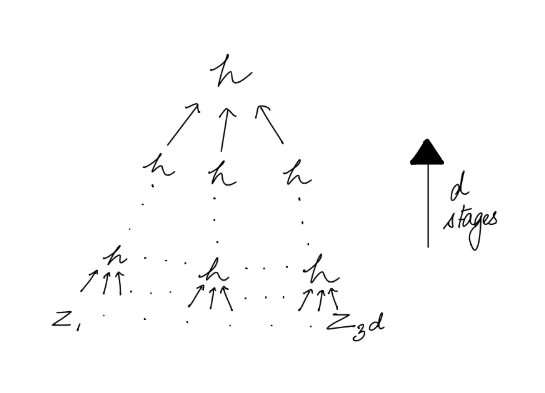
\includegraphics[width=0.5\textwidth]{H_d-tree}
\caption{The tree depicting the function $H_d(z_1, ... ,z_{3^d})$ obtained from the iterated construction using the gadget $h(z_1, z_2, z_3)$ } \label{fig:H_d-treel}
\end{figure}
\noindent $H_d(\text{all 0s}) \rightarrow 0$ and $H_d(\text{exactly one 1}) \rightarrow 1$ and the other cases are irrelevant as the function is allowed to return anything when the condition for \emph {Unique Set Disjointness} is violated. \newline

\noindent $\therefore H_d(z_1, ... z_{3^d}) = 
     \begin{cases}
       \text{0} &\quad{if\; z_1 + ... + z_{3^d} = 0} \\
       \text{1} &\quad{if\; z_1 + ... + z_{3^d} = 1} \\
       \text{?} &\quad{otherwise}\\
     \end{cases}
$ \newline 

\noindent Define $f (x, y) = H_d(\text{the bitwise conjunction of x with y}) = H_d(x \wedge y)$\newline

\noindent $\therefore n = 3^d$ and $d = log(n)$\newline

\noindent Using Fact 5.7, it is known that a problem that belongs to this family must have $D(f) = \Omega(n) = \Omega(3^d)$\newline

\noindent Now we must show that the rank of the characteristic matrix $M_f$ is small despite the function having high communication complexity. \newline

\noindent $rk M_f = rk[h(x \wedge y)]_{x, y \in {\{0, 1\}}^{3^d}}$ \newline

\noindent $\therefore$ Consider the case where d = 1 \newline

\noindent But $rk M_f = rk [x_1y_1 + x_2y_2 + x_3y_3 - x_1x_2y_1y_2 - x_1x_xy_1y_2 - x_2x_3y_2y_3] = rk [x_1y_1] + rk [x_2y_2] + rk[x_3y_3] - rk[x_1x_2y_1y_2] - rk[x_1x_xy_1y_2] - rk[x_2x_3y_2y_3]$\newline

\noindent The rank of each of matrix in the sum above is $\leq 1$ (as each of the matrix is filled with 0s except for the terms where both x and y meet the condition and thus there can be at most 1 linearly independent row or column) $\implies rk M_f \leq 6$ for d = 1\newline

\noindent But similarly in the general case, $rk M_f \leq$ the number of monomials in $H_d(z_1, ...,, z_{3^d})$. \newline

\noindent Inductively it is easy to see that the the number of monomials in $H_d(z_1, ...,, z_{3^d}) \leq 6^{2^{d} -1}$. (After having the proven the base case for d = 1, this inequality can be conjectured for d = k - 1 and using identically the formula for $h(z_1, z_2, z_3)$ it can be shown to hold true inductively for d = k and hence must be true for all d $\in \mathbb{Z}^+$ \newline

\noindent Hence, to conclude $D(f) \geq \Omega(3^d) = \Omega{(log(6^{2^d}))}^{log(3)} \implies D(f) \geq \Omega{(log(rkM_f))}^{log(3)}$. QED 

\end{proof}

\section{Solution to Challenge Problem 6}

\begin{problem}
Prove $$ D(f) \leq rk M_f + 1 $$ for any function $f: {\{0, 1\}}^n \times {\{0, 1\}}^n \rightarrow \{0, 1\}$
\end {problem}

\begin{proof}
The main idea behind this solution is to prove a stronger statement using a field like $F_2$ which is far easier to work in than $\mathbb{R}$ \footnote {It is assumed that when the field is not specified the rank being referenced is over $\mathbb{R}$} and use lemma 5.1 to trivially complete the proof for the original statement. Moreover, the way to prove any upper bound on the communication complexity of a problem is by showing a protocol that achieves this complexity. Thus the proof below outlines a protocol that achieves the desired upper bound. \newline

\noindent Let r = $rk_{F_2} M_f$ \newline

\noindent This implies that there exist r linearly independent rows (or equivalently columns)  $v_1, v_2$, ... ,$v_r$ such that every row in $M_f$ is a linear combination of these r vectors \newline

\noindent Note that the rows of $M_f$ represent the possible inputs for Alice and hence for Alice to convey which row she has to Bob is equivalent to conveying her entire input. \newline

\noindent But since any row that corresponds to Alice's input can be represented as a linear combination of the r vectors and since the field being worked on is $F_2$ each co-efficient can be expressed in a single bit, it takes only r bits of communication for Alice to indicate what her input is to Bob. \newline

\noindent As a result, Bob can compute the final answer and send back the final answer bit. \newline

\noindent The total cost of this protocol was r + 1 bits but r = $rk_{F_2}(M_f)$ and $rk_{F_2}(M_f) \leq rk{M_f}$  by lemma 5.1 \newline

\noindent Hence $D(f) \leq rk M_f + 1$. QED 
\end{proof}

\bibliographystyle{abbrv}
\bibliography{template}

\end{document}
